%%%%%%%%%%
% HEADER %
%%%%%%%%%%

\documentclass[
  10pt, 
  a4paper,
  oneside, 
  % twoside, 
  headinclude, 
  footinclude, 
  BCOR5mm, 
]{scrartcl}

% package
\usepackage[francais]{babel}
\usepackage{color}
\usepackage{enumitem}

\usepackage{minted}
\usemintedstyle{trac}
\definecolor{LightGray}{gray}{0.90}

\usepackage[pdftex]{graphicx}

\setlength{\parindent}{0cm}
\setlength{\parskip}{1ex plus 0.5ex minus 0.2ex}
\newcommand{\hsp}{\hspace{20pt}}
\newcommand{\HRule}{\rule{\linewidth}{0.5mm}}

\fvset{
  frame = lines,
  framesep = 2mm,
  baselinestretch = 1,
  rulecolor = \color{LightGray},
  fontsize = \normalsize,
  tabsize = 3,
}

%%%%%%%%%%%%%%%%%%%%%%%%%%%%%%%%%%%%%%%%%
% Arsclassica Article
% Structure Specification File
%
% This file has been downloaded from:
% http://www.LaTeXTemplates.com
%
% Original author:
% Lorenzo Pantieri (http://www.lorenzopantieri.net) with extensive modifications by:
% Vel (vel@latextemplates.com)
%
% License:
% CC BY-NC-SA 3.0 (http://creativecommons.org/licenses/by-nc-sa/3.0/)
%
%%%%%%%%%%%%%%%%%%%%%%%%%%%%%%%%%%%%%%%%%

%----------------------------------------------------------------------------------------
%	REQUIRED PACKAGES
%----------------------------------------------------------------------------------------

\usepackage[
nochapters, % Turn off chapters since this is an article        
beramono, % Use the Bera Mono font for monospaced text (\texttt)
eulermath,% Use the Euler font for mathematics
pdfspacing, % Makes use of pdftex’ letter spacing capabilities via the microtype package
dottedtoc % Dotted lines leading to the page numbers in the table of contents
]{classicthesis} % The layout is based on the Classic Thesis style

\usepackage{arsclassica} % Modifies the Classic Thesis package

\usepackage[T1]{fontenc} % Use 8-bit encoding that has 256 glyphs

\usepackage[utf8]{inputenc} % Required for including letters with accents

\usepackage{graphicx} % Required for including images
\graphicspath{{graphics/}} % Set the default folder for images

\usepackage{enumitem} % Required for manipulating the whitespace between and within lists

\usepackage{lipsum} % Used for inserting dummy 'Lorem ipsum' text into the template

\usepackage{subfig} % Required for creating figures with multiple parts (subfigures)

\usepackage{amsmath,amssymb,amsthm} % For including math equations, theorems, symbols, etc

\usepackage{varioref} % More descriptive referencing

%----------------------------------------------------------------------------------------
%	THEOREM STYLES
%---------------------------------------------------------------------------------------

\theoremstyle{definition} % Define theorem styles here based on the definition style (used for definitions and examples)
\newtheorem{definition}{Definition}

\theoremstyle{plain} % Define theorem styles here based on the plain style (used for theorems, lemmas, propositions)
\newtheorem{theorem}{Theorem}

\theoremstyle{remark} % Define theorem styles here based on the remark style (used for remarks and notes)

%----------------------------------------------------------------------------------------
%	HYPERLINKS
%---------------------------------------------------------------------------------------

\hypersetup{
%draft, % Uncomment to remove all links (useful for printing in black and white)
colorlinks=true, breaklinks=true, bookmarks=true,bookmarksnumbered,
urlcolor=webbrown, linkcolor=RoyalBlue, citecolor=webgreen, % Link colors
pdftitle={}, % PDF title
pdfauthor={\textcopyright}, % PDF Author
pdfsubject={}, % PDF Subject
pdfkeywords={}, % PDF Keywords
pdfcreator={pdfLaTeX}, % PDF Creator
pdfproducer={LaTeX with hyperref and ClassicThesis} % PDF producer
}

\hyphenation{Fortran hy-phen-ation}

\titleformat
  {\section}[block]
  {\sffamily\large\normalfont}
  {\thesection}
  {1em}
  {\Large\spacedlowsmallcaps}

\titleformat
  {\subsection}[block]
  {\sffamily\normalsize\normalfont}
  {\thesubsection}
  {1em}
  {}

% STYLE

\renewcommand{\sectionmark}[1]{\markright{\spacedlowsmallcaps{#1}}}
\lehead{\mbox{\llap{\small\thepage\kern1em\color{halfgray} \vline}\color{halfgray}\hspace{0.5em}\rightmark\hfil}}

\pagestyle{scrheadings}
\setcounter{tocdepth}{3}


% HEAD PAGE

\begin{document}

%\maketitle

\begin{titlepage}
  \begin{sffamily}
  \begin{center}
    \textsc{\LARGE Université de Fribourg} \\ [2cm]
    \textsc{\Large Very Deep Learning} \\ [2cm]

    % Title
    \HRule \\ [0.5cm]
    {\huge\spacedallcaps{Deepdraw} \\ [0.5cm]}
    \HRule \\ [2cm]
    
    \textsc{
    	\Large Ismaïl \spacedallcaps{Senhaji}, 
    	\Large Gil \spacedallcaps{Clavien} \\
    	\Large Noé \spacedallcaps{Zufferey}, 
    	\Large Michaël \spacedallcaps{Diatta} \\
    	\Large Igor \spacedallcaps{Dundic}} \\ [2cm]
    
    \textsc{\large \emph{Responsable} : Marcus \spacedallcaps{Liwicki}} \\ [0.5cm]
    \textsc{\Large 20 décembre 2017} \\    

    \vfill

    % Bottom of the page
    Département d’Informatique — Departement für Informatik \\
    Université de Fribourg — Universität Freiburg \\
    Boulevard de Pérolles 90, 1700 Fribourg, Suisse
  \end{center}
  \end{sffamily}
\end{titlepage}

\newpage

% CONTENT

\section{Introduction}

For the very deep learning project, we decided to build, train and manage a neural network that can draw pictures of simple concept. We use the Quick Draw Dataset, a google's game, that provide a huge dataset of labelised simple drawing.

\section{About quickdraw-dataset}

The Quick Draw Dataset\footnote{\url{https://github.com/googlecreativelab/quickdraw-dataset}} is a collection of 50 million drawings across 345 categories, contributed by players of the game Quick, Draw!\footnote{\url{https://quickdraw.withgoogle.com/\#}}. The drawings were captured as timestamped vectors, tagged with metadata including what the player was asked to draw and in which country the player was located.

The Quick Draw game principle is to draw specific picture given by the computer. This one try to recognize, with machine learning, your drawing.

\begin{figure}[h]
	\center
	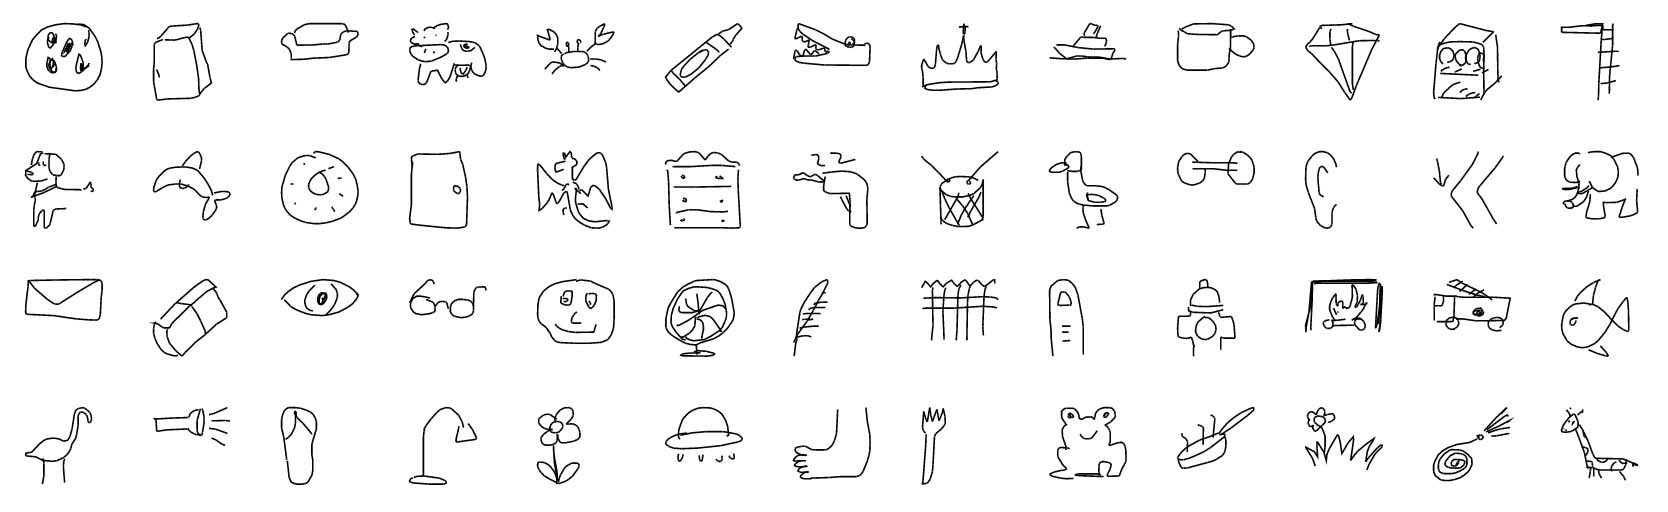
\includegraphics[width=\columnwidth]{qdd-example.jpg}
	\caption{Quick Draw example.}
	\label{promo-asylamba}
\end{figure}

The Quick Draw Dataset provides preprocessed dataset. We choose to use the \textbf{Simplified Drawing files} preprocessed dataset. They've simplified the vectors, removed the timing information, and positioned and scaled the data into a 256x256 region. The data is exported in ndjson format with the same metadata as the raw format. We use a binary version of this format, for efficiency purpose.


\section{Goals}

The final goal of this project is to reverse the principle given in the previous section: with give a class to the computer and this one try to draw the corresponding drawing.


\section{Deepdraw code}

Présenter les choix, les NN et tout ce merdier

\subsection{Get the data}

The size of the dataset presented an interesting challenge: at 7.1GB in the
packed binary format, and even more once parsed into Python data types, it
barely fits into memory. To solve this, we build an index file containing each
drawing's id, class (and by extension the file where it can be found), and its
offset within the file. The size of the resulting \texttt{index.csv} file is
1.6GB, small enough to be loaded into memory in a reasonable time.

Drawings are provided as a sequence of strokes, where each stroke is a sequence
of $(x, y)$ coordinates. This format isn't particularly suited for a Neural
Network, thus the need to transform them. We implemented a \texttt{Rasterizer}
class, responsible for converting such a sequence of strokes to a 256 by 256
rasterized image, using Bresenham's line
algorithm\footnote{\url{https://en.wikipedia.org/wiki/Bresenham\%27s_line_algorithm}}.
This class is compatible with Torch's transormation framework and can be used in
conjunction with other transformations, such as resizing or normalizing the image.

Another transormation class was implemented, \texttt{Sequencer}, which converts
the drawing into a sequence of state vectors, for use in a Recurrent Neural
Network\footnote{\url{https://arxiv.org/abs/1704.03477}}. This approach wasn't
used, however.

\subsection{First NN: GAN}

Generative aversarial networks called GANs belong to the familly of generative models. Which we can define as a familly of model that takes a dataset containing samples from a distribution $p_data$ and learns in someway to represents this distribution $p_model$. In this project we will judge the quality of this representation by generating some samples of $p_model$.

We choose to focus our work on generative models and GANs in particular because it's an interesting way to test our capacity to represent and play with the probability distribution of drawing ability of humans. The question is: can a model draw realistic samples of an object (an apple for example) as a human can do it, considering the high variability of the samples.

GANs can represent the samples distribution by using a Maximum likelihood estimation, this means that we choose some parameters for our model that maximize the likelihood of the training data, in a log space, because of numerical issues correlated to computers design.

\subsubsection{GAN framework}
The framework is made of two parts. There is on generator that creates samples that belongs to $p_model$ but which should come from the same distribution as the training set $p_data$. The other part consist of a discriminator.

\begin{figure}[!h]
  \makebox[\textwidth][c]{
    \subfloat[Epoch 55.]{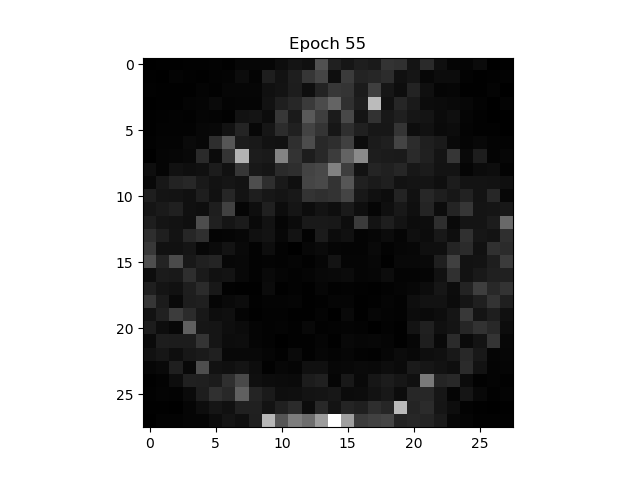
\includegraphics[width=.45\columnwidth]{apple-sample-57}}\quad
    \subfloat[Epoch 75.]{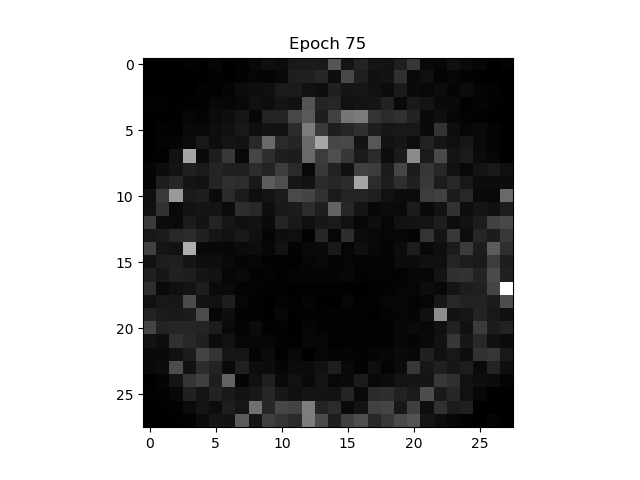
\includegraphics[width=.45\columnwidth]{apple-sample-75}}\quad
    \subfloat[Epoch 115.]{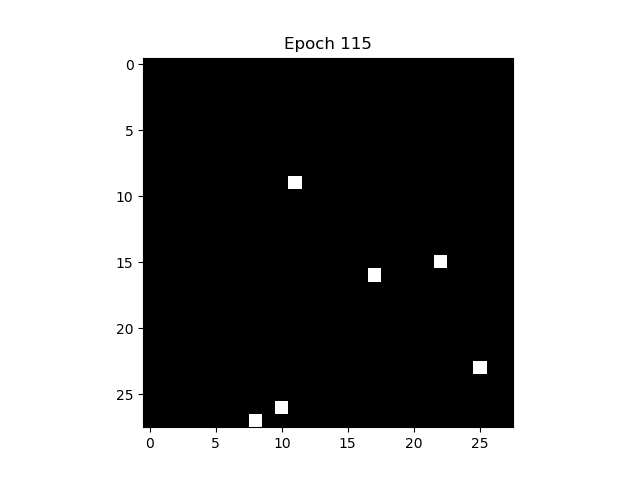
\includegraphics[width=.45\columnwidth]{apple-sample-115}}
  }
  \caption{Légende TODO}
  \label{s1-anaylse-v2}
\end{figure}

\subsection{Second NN: DCGAN}

Discriminative...

\begin{figure}[!h]
  \makebox[\textwidth][c]{
    \subfloat[Epoch 9.]{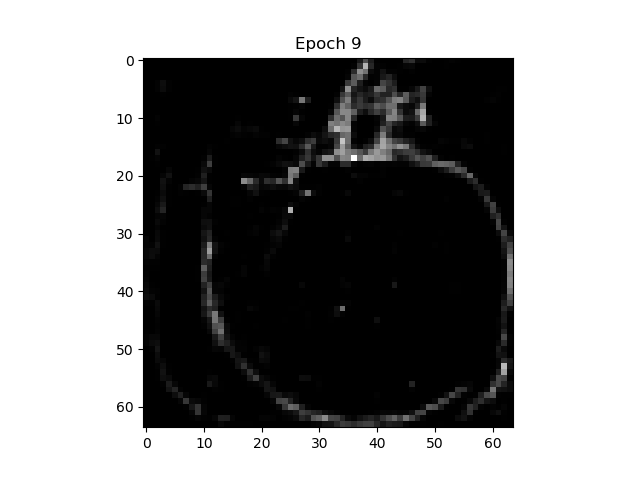
\includegraphics[width=.90\columnwidth]{apple-dc-sample-9}}\quad
    \subfloat[Epoch 21.]{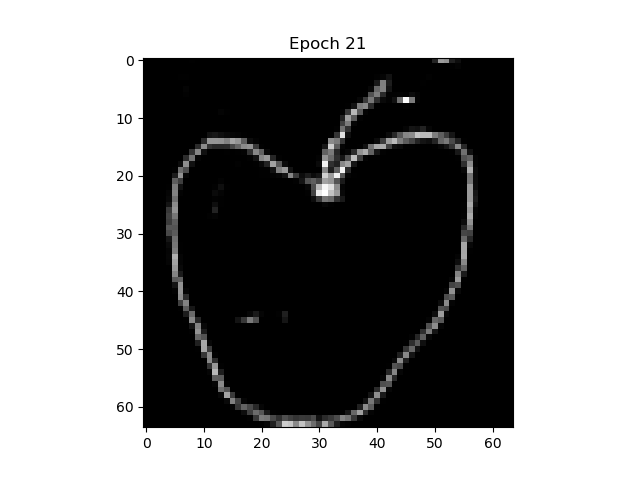
\includegraphics[width=.90\columnwidth]{apple-dc-sample-21}}\quad
  }
  \caption{Légende TODO}
  \label{s1-anaylse-v2}
\end{figure}


\section{Problems}

Les problèmes qu'on a eu, outre les problèmes de natel de Mick...


\section{Résultat}

On présente les résultats et on nique des mères... histoire de fêter ça...


\section{Further work}

Warsserstein

WaffenSS


\newpage

\tableofcontents
\listoffigures
\listoftables

\begin{thebibliography}{9}
\end{thebibliography}
\end{document}